\cleartooddpage[\thispagestyle{empty}]
\chapter{Gamma Ray Reconstruction}\label{ch:grrecon}

In chapter \ref{chapter:veritas}, it was explained how the trigger system preserves PMT voltage traces of potential events.
To reconstruct gamma rays, the voltage traces caused by cherenkov photons must be identified and combined to form an image of the original cherenkov shower.
Then the shower images from multiple telescopes can be used to reconstruct the original gamma ray's energy and direction.

\section{Pedestal Variation}
Before reconstructing any events, the pedestal and pedestal variations must be calculated.
These are done by artificially triggering all pixels once per second during normal data-taking, in order to record events that solely contain noise.
The average of the digital counts (dc) of all noise-events for each pixel is then the pedestal.
From this pedestal, the pedvar is then calculated as the rms of the all the dc counts in all noise-events, which can be visualized as the distribution of dc around the mean dc.

(also see \cite{Hanna2010NIM} about relative gains??)

\section{Pixel Identification}
The first step is to determine which pixels are part of a shower image or not.
This is done by subtracting the digital counts pedestal from the entire trace, and then integrating the total dc in each voltage trace.
In addition, the time when the voltage trace is at half of its maximum value, called $T_{0}$.

Around time $T_{0}$, the trace is integrated a second time with a smaller time window (usually either 14 or 24 ns wide, 30\% of the window before $T_0$), to reduce the inclusion of dc from sources of noise (NSB and electronics).
This two-pass algorithm is usually referred to as the double-pass method (cite??).
If a pixel's second-pass total dc is higher than 5 times the pedvar, then it is considered an image pixel.
If it is between 2.5 and 5 times the pedvar, it is considered a border pixel.

Once all pixels have been classified, isolated border pixels that have no neighboring image pixel are also removed, as they are more likely to be due to noise than cherenkov photons.
Then, the time gradient from the image and border pixels can be found by examining a linear fit of the $T_{0}$ times.
This gradient can then be used to place a third integration integration window with 30\% of the window before each pixel's $T_{0}$, to more accurately measure the charge due to cherenkov photons in the pixel.

From the image pixels, border pixels, and time gradient, the shower's Hillas parameters can be calculated.
These include the size of the shower in photoelectrons (or equivalent units), the shower center of charge, angle, length and width.
The center of charge is the charge-weighted average of all image and border pixel positions.
The angle of the shower determines how the image's major axis is oriented in the camera.
The shower length and width are determined by the rms of the shower image along its major and minor axes, respectively.


\section{Position Reconstruction}\label{subsec:posrecon}
By examining the images from multiple telescopes, the initial position of the event can be determined.
This is done by overlapping all telescope images in a single camera coordinate system, and projecting each image's major axis backwards in time.
These drawn lines should intersect very close together, and a weighted average of the intersection points determines the event's initial direction.

In averaging the intersection points, weighting for each intersection can be applied based on the angle between the two lines.
This improves the reconstruction, because the intersection point from two images at 90\degree angles will be less sensitive to image fluctuations than two images at 160\degree, as shown in figure \ref{fig:largeintersectangle}.
Additionally, the disp method can be utilized to offer improvements in the lower elevations.

\begin{figure}[ht]
  \begin{center}
    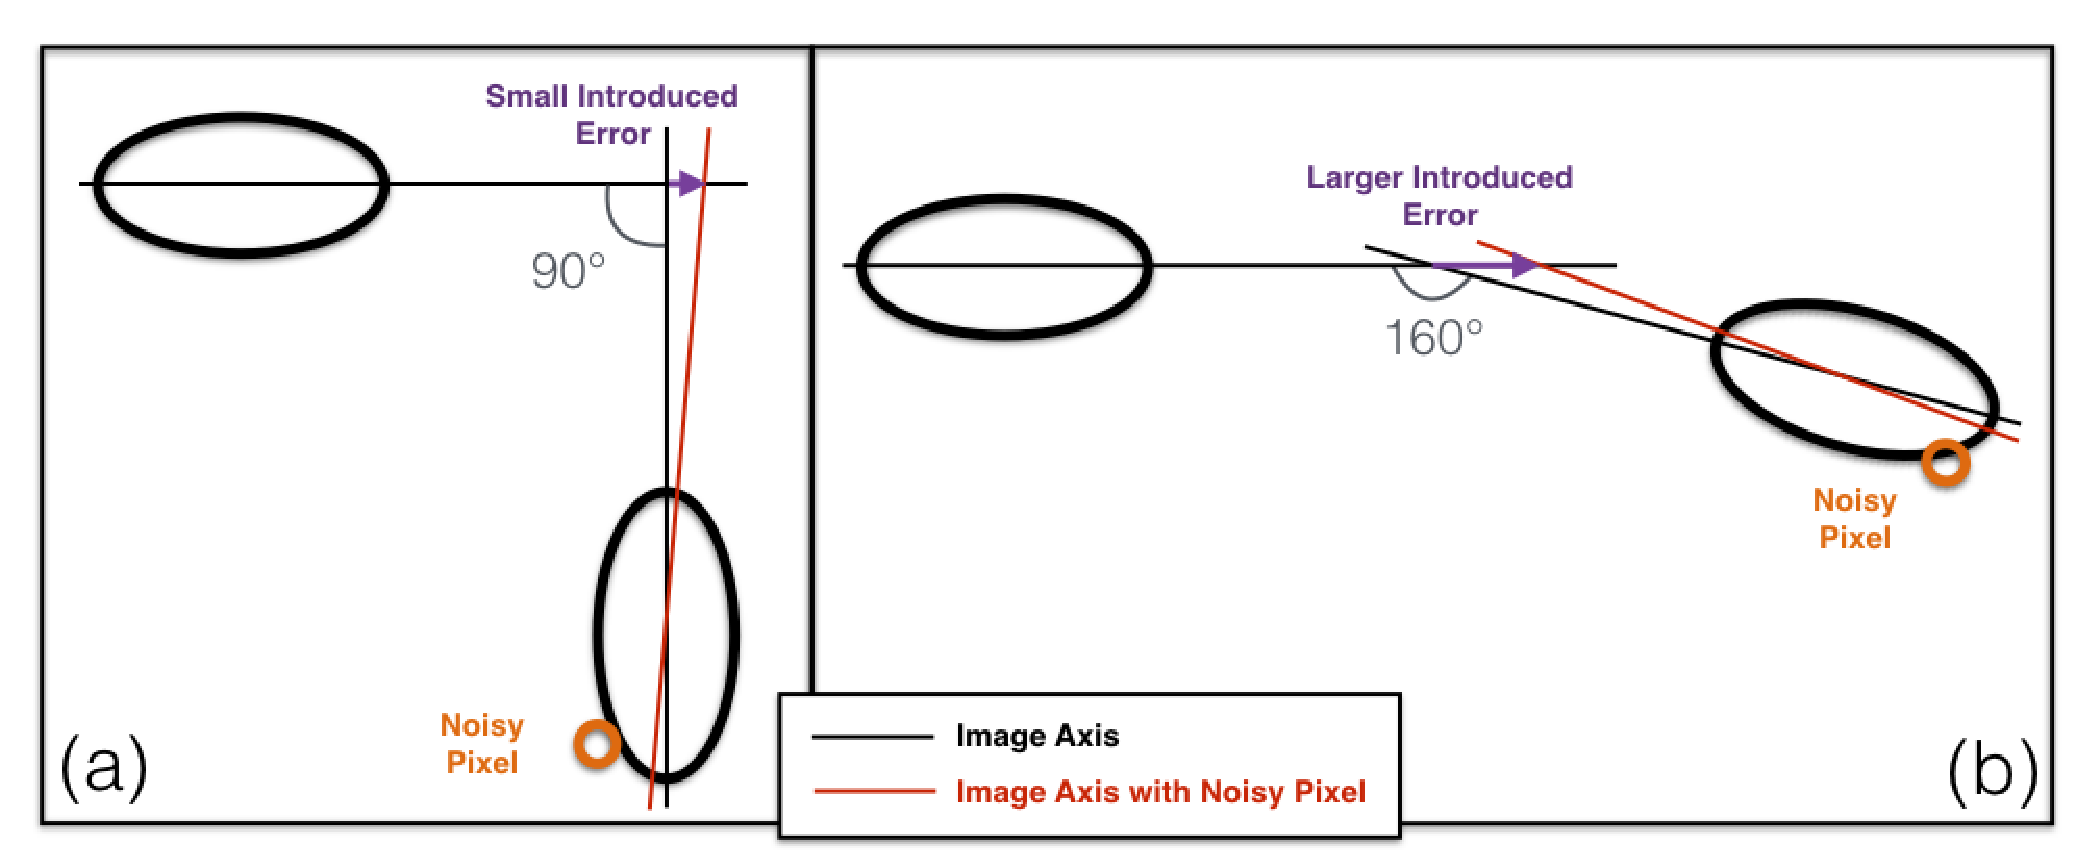
\includegraphics[width=0.95\textwidth]{images/large_angle_image_intersection_error_cropped.eps}
    \caption[Large Image Intersection Angles]{In diagram (a), when a noisy pixel is added to an image, the reconstructed position is only moved a small distance (the purple arrow).  In diagram (b), due to the large angle between images, the reconstructed position is much larger.}\label{fig:largeintersectangle}
  \end{center}
\end{figure}

\subsection{Angular Reconstruction Neural Network}\label{subsec:disp}
At high elevations, shower images are often at large intesection angles, because the telescopes are spread out in two dimensions, relative to the shower in the atmosphere.
At low elevations near the galactic center, however, the telescope array flattens into one dimension, which makes the shower's impact parameter (the shortest distance between the telescope and the shower core axis) smaller for two of the telescopes.
These two closer telescopes then have very short, almost circular images, which increases the sensitivity of those two image axes to noisy pixels or shower fluctuations, as shown in figure \ref{fig:showerhighlowelev}.
This also causes the remaining telescope images to have large intersection angles, which also reduces the accuracy of the position reconstruction.

\begin{figure}[ht]
  \begin{center}
    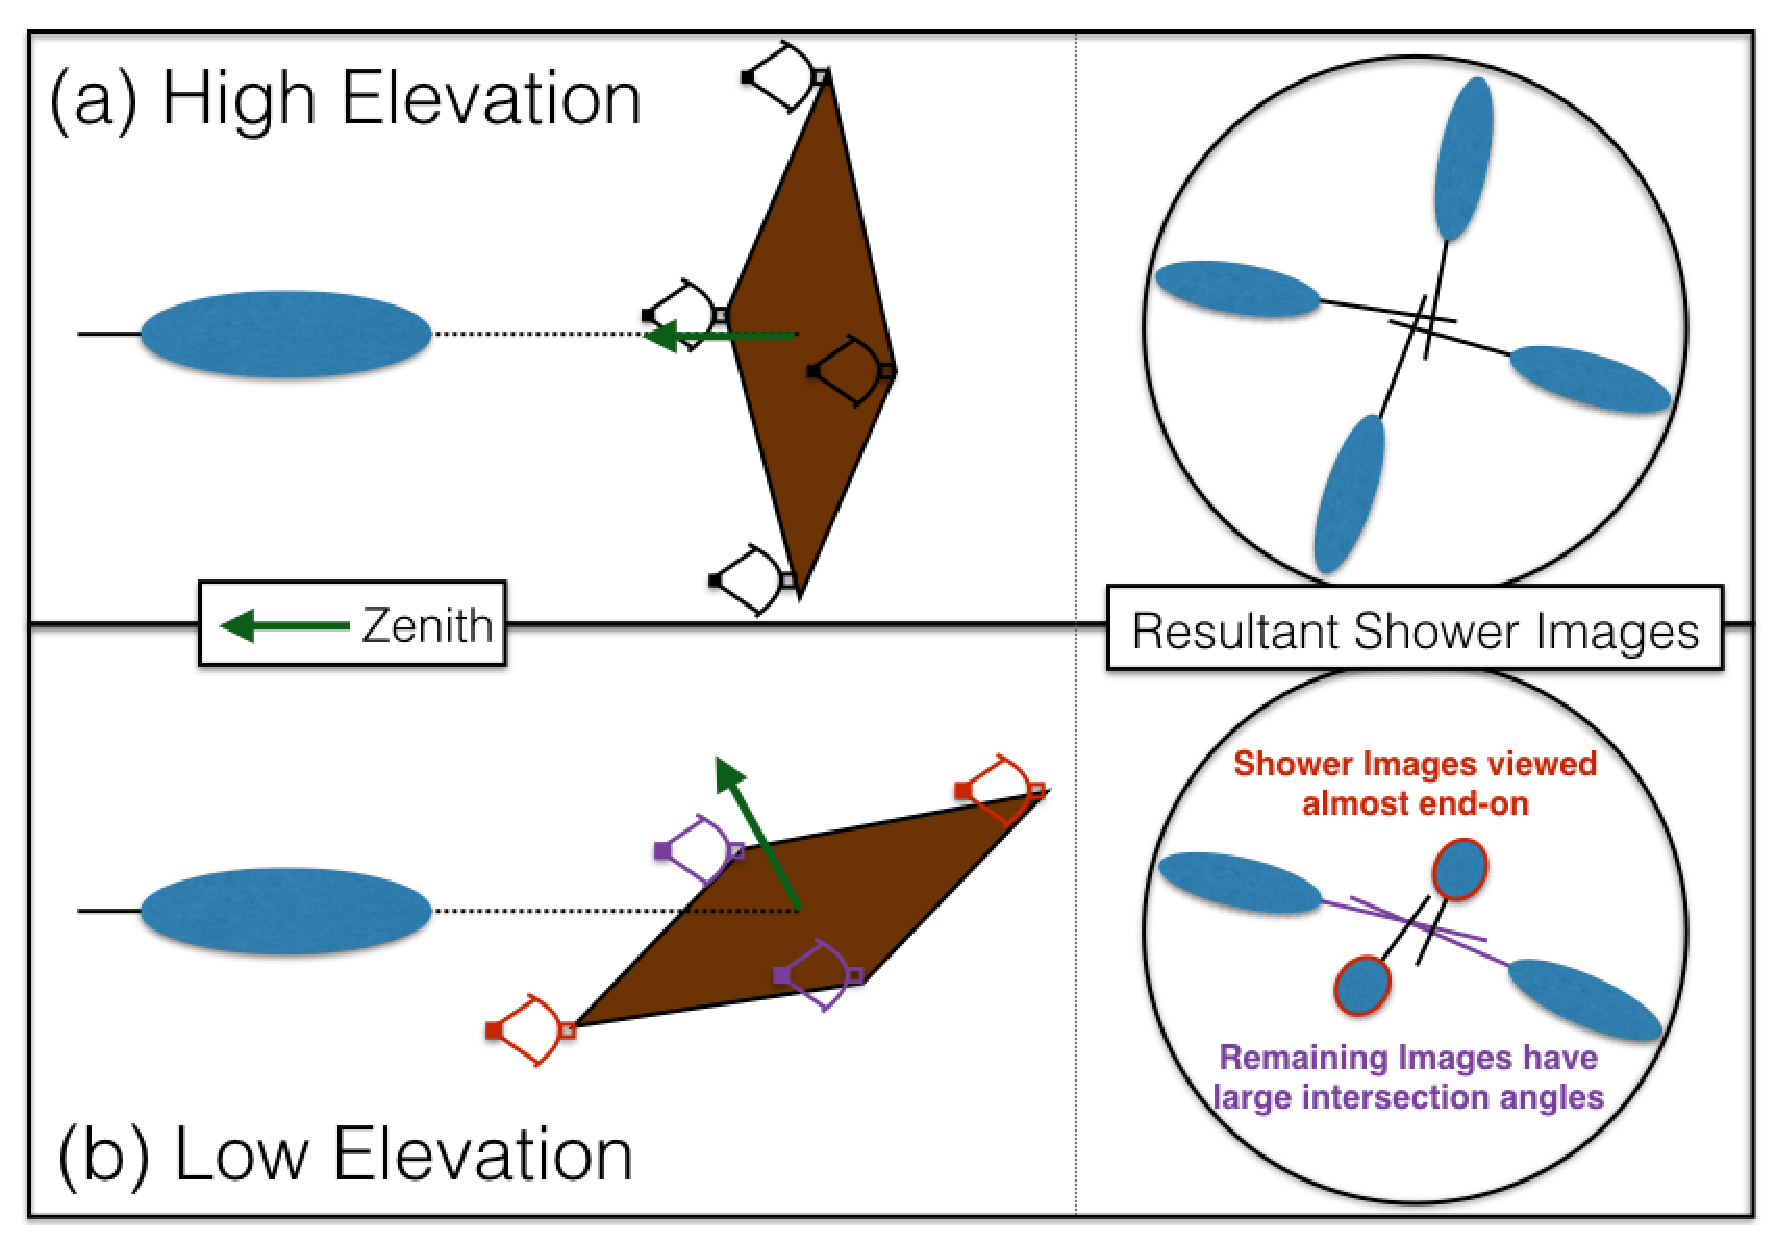
\includegraphics[width=0.75\textwidth]{images/high_elevation_vs_low_shower_images_cropped.eps}
    \caption[Shower Images at High and Low Elevations]{In figure (a), high elevation showers produce long images in all four telescopes.  In figure (b), lower elevation showers produce shortened images in two telescopes, and the remaining images form large angle intersection.}\label{fig:showerhighlowelev}
  \end{center}
\end{figure}


To better handle these near-parallel image axes at low elevations, the reconstructed position can be determined from more parameters than just the weighted image axes intersection points.
From simulations, the distance between the center of the hillas shower image and the reconstructed position can be calculated, where the angular distance between the two is the 'disp' parameter\cite{Senturk:2011}, shown in figure \ref{fig:dispdiagram}.
Then, a machine learning algorithm \cite{Beilicke2012NIM} can be trained on these simulations at various energies and positions in the camera(??).
This algorithm's disp-predicted positions can then be weighted and included in the intersection averaging.

\begin{figure}[ht]
  \begin{center}
    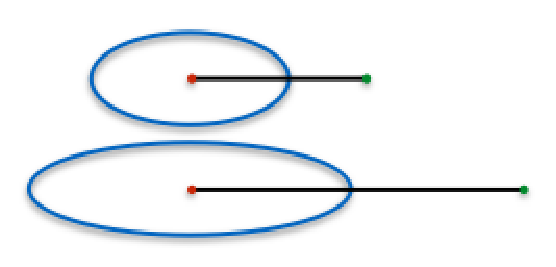
\includegraphics[width=0.5\textwidth]{images/disp_parameter_cropped.eps}
    \caption[Angular Reconstruction Disp]{The disp parameter is the angular distance between the center (red dot) of a hillas image (blue oval) and the true sky position (green dot).  Generally, longer shower images have a larger disp angle.}\label{fig:dispdiagram}
  \end{center}
\end{figure}

% https://veritas.sao.arizona.edu/wiki/index.php/BDT_Angular_reconstruction
The disp and other parameters for thousands of simulated showers can then be used to train a boosted decision tree forest (BDT) that estimates the most probable disp for a given shower.
This most probable disp can then be used with the image axes intersection points to more accurately reconstruct the original gamma-ray point of origin.

Once the training is complete, it is tested on a separate set of 17,000 simulated events, which are plotted in figure \ref{fig:disptraining}.
The x axis describes the true disp value for each event, while the y axis describes the disp value estimated by the BDT, with a black line for the x=y line, which represents a perfect disp reconstruction.
As the majority of the events fall on the line, it can be concluded that the BDTs are able to predict the correct disp value for most images.

% made from screenshot of last slide in Dropbox/Presentations/20160719_Group_Meeting.key
\begin{figure}[ht]
  \begin{center}
    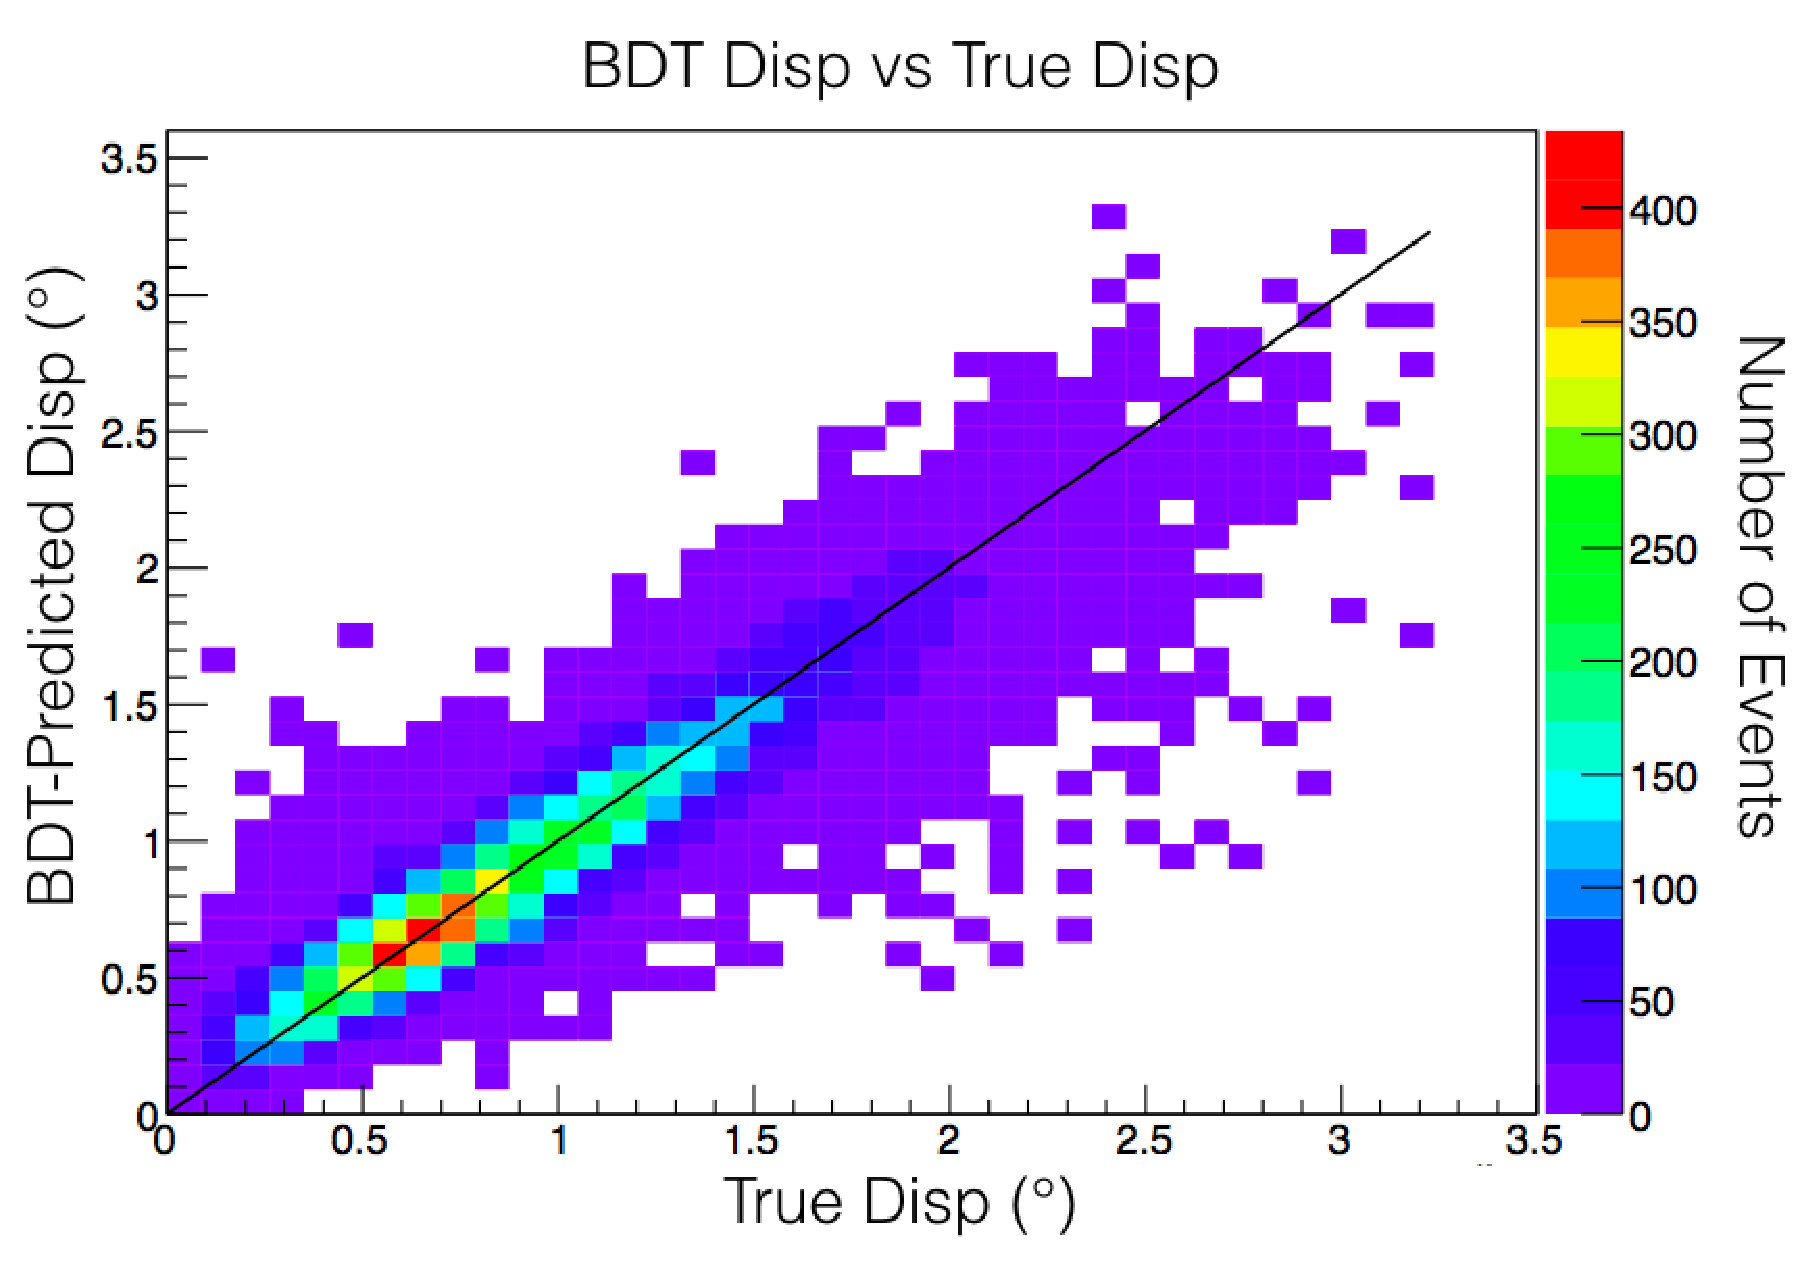
\includegraphics[width=0.85\textwidth]{images/disp_training.eps}
    \caption[Disp BDT Training]{The true disp vs the BDT-predicted disp, for \nicetilde17,000 gamma-ray event images in T1, from 500GeV to 200TeV.}\label{fig:disptraining}
  \end{center}
\end{figure}

The small improvement in the position reconstruction due to the disp method can be seen in figure \ref{fig:disp_event_offset}.
With the Geometric (red) events, more are concentrated further from the point source, while with the Disp method, somewhat more are concentrated at the source itself.

\begin{figure}[ht]
  \begin{center}
    \includegraphics[width=\textwidth]{images/disp_event_offset_hists/disp_event_offset_hist.eps}
    \caption[DISP Offset Improvement]{The number of events at different angular offsets from the Crab and the Galactic Center, with both Geometric and Disp reconstruction methods.}\label{fig:disp_event_offset}
  \end{center}
\end{figure}


\section{Energy Reconstruction}\label{subsec:enrecon}
To reconstruct the energy of each shower, a database of simulated showers is built.
This database includes the width and length of the shower, how far away its core position is, how bright it was, as well as its reconstructed and true energy.
By scanning through this database for showers that are similar to the one being constructed, the most similar-looking shower then indicates the true energy(??).



\section{FITS Conversion for Gammalib and CTOOLs}

Once gamma rays have been reconstructed with event display, they must be converted to a FITS file format compatible with Gammalib and Ctools.
This format consists of a FITS file with an event list table, containing each gamma ray, its energy, sky direction, and time.
This also includes meta information about the event list like the telescope's pointing target and the start and end times of the event list.
This FITS file can then be read into Gammalib and CTOOLS \cite{gammalibctools}.

In addition to the event list, the instrument response functions (IRFs) must also be imported into Gammalib and Ctools.
These include effective areas, point spread functions, energy dispersion, and background models for several dimensions in the IRF parameter space (energy, offset from camera center, telescope elevation/azimuth, NSB noise, etc).
By default, all IRFs are stored in a single database, and each event list contains a reference to which part of the parameter space should be used with it.

However, the galactic center is at an elevation of $\ang{30}$, much lower than most VERITAS observation targets.
At this elevation, with its field of view of $\ang{3.5}$, the air mass column density ($g/cm^{2}$) is 20\% higher at the bottom of the camera than at the top.
Add to this that during a single 30 minute observation, the elevation of the Galactic Center can change by several degrees, means the airmass in view of the camera may change rapidly, meaning the IRFs may become time dependent.

To allow for the inclusion of this time dependence in the analysis, an alternate way of storing the IRFs was chosen, diagrammed in figure \ref{fig:fits_scheme}.
First, one observation (typically 20-30 minutes long) is broken up into \nicetilde8 minute chunks.
Each chunk is then converted to an event list, and saved to a FITS file.
In addition, the needed Effective Area, PSF, and background models are also written to the same FITS file.
As each event list covers a small region in time, the IRF tables only need to contain the dimensions of the parameter space that can change during one chunk, such as event energy and distance from camera center.

\begin{figure}[ht]
  \begin{center}
    \includegraphics[width=0.75\textwidth]{images/FITS_diagrams_alternate_scheme.eps}
    \caption[FITS File Event Storage Schemes]{}\label{fig:fits_scheme}
  \end{center}
\end{figure}

The end result is that a 30 minute observation can be broken into several FITS files (called chunks), where each chunk file is independent of any outside references, contains all needed IRF information, and only takes up \nicetilde100s KB on disk.
This makes it ideal for an analysis program to automatically download any needed data over an internet connection, as each chunk is tiny and has no outside dependencies.
As gammalib and CTOOLS expect the default FITS file scheme, a python function was written to automatically load all event and irf tables from a single fits file, and import this information into gammalib's GObservation class.

There were minor issues with converting the IRFs that are noted in the following sections.

\subsection{Effective Area}\label{sec:effarea}
% plot of effective area vs energy
Effective area is the measure of how large an observatory's collection area is, determining how many gamma rays are be detected per unit time, solid angle, and energy.

For each point in the parameter space, the effective areas are calculated with many Monte Carlo gamma ray simulations.
This is done in the shower plane, the plane perpendicular to the line drawn between an observing source, and the center of the observatory.
The effective area is then calculated via:
$A=\pi R^2 \frac{N_{survived}}{N_{simulated}}$
where R is the radius of the area within which simulated showers are directed to fall, $N_{simulated}$ is the number of showers that were initially simulated into the area, and $N_{survived}$ is the number of simulated showers that pass all cuts.
This 'Effective' area is thus a measure of how much detection area the observatory would have if it had a 100\% detection efficiency, which can then be used in calculating a source's flux.

\begin{figure}[ht]
  \begin{center}
    \includegraphics[width=0.75\textwidth]{images/effarea_plots/effarea_parameter_space.eps}
    \caption[Effective Area Parameter Space]{Effective areas at different points in the Energy and Camera Offset parameter space for run 78128.}\label{fig:effarea_paramspace}
  \end{center}
\end{figure}

For the test analyses of the Crab and the Galactic Center Point Source, the effective areas of all events are shown in figure \ref{fig:effarea_usage}.

\begin{figure}[ht]
  \begin{center}
    \includegraphics[width=\textwidth]{images/effarea_plots/effarea_usage.eps}
    \caption[Effective Area Parameter Space]{Effective Areas used by events in each analysis.}\label{fig:effarea_usage}
  \end{center}
\end{figure}

\subsection{Point Spread Function}\label{sec:psf}

In addition to the energy being slightly mis-reconstructed, the source position of the gamma ray can also be misreconstructed.
For VERITAS, this misreconstructions are measured by simulating many gamma rays in the camera, and looking at the distribution of true positions for a given reconstructed position, which is called the point spread function (PSF).
To first order, most current-generation point spread functions are gaussian distributions.
For Event Display, the PSF has been roughly measured to be gaussian-shaped.
For CTOOLS instead, a King function (Eqn \ref{eqn:king}) was fitted to the distribution of events, as Fermi and HESS have found (cite??) gamma ray PSFs tend to have longer tails than a Gaussian, which the king function better handles.

The psf is the distribution of true event directions for a given reconstructed event direction.
Within an analysis, the event PSF strongly depends on the event energy, as well as its distance from the camera center.

In order to use Event Display's psf in ctools, some conversion is necessary.
Event display natively stores its psf as a pair of 68\% and 80\% containment radii (referred to as $r_68$ and $r_80$, respectivly), each as a distance in degrees between the monte carlo event direction and the reconstructed direction.
These radii contain 68\% and 80\% of all events in the distribution, and are used to fit a gaussian profile.
For ctools, a king function is used instead of a gaussian.

\begin{equation} \label{eqn:king}
$$ psf_{king}(r) = \frac{1}{2 \pi \sigma^{2} } \left( 1 - \frac{1}{\gamma} \right) \left( 1 + \frac{ r^{2} }{ 2 \gamma \sigma^{2} } \right)^{-\gamma} $$
\end{equation}

where $r$ is the angular distance from the reconstructed position, $\sigma$ is similar to the width of a gaussian , and the $\gamma$ parameter affects how long the tails are.
The function is integrates to 1 in polar coordinates with $r$ in radians.

A king function fitting algorithm was added, that fits for the $\gamma$ and $\sigma$ parameters, from the same distribution of events that the r68 and r80 radii are calculated from.
This leads to good fits over almost all of the parameter space.

(example fit image of distribution of events and fitted king function ??)

A smaller psf is important for this analysis, as the presence of a dark matter halo relys on the pointing accuracy of the events around the galactic center.
A worse gamma-ray psf (with a wider distribution of possible true positions) will smear out any dark matter halo around the galactic center, making its detection more difficult.

In figure \ref{fig:psf_paramspace}, the psf is shown for one Galactic Center run.
In it, one can see how the psf containment radius changes vs reconstructed energy and offset from the camera's center.
Other runs, which have different elevations, azimuths and NSB noise levels will have different values at each point in the energy/offset parameter space.

% plot of psfs from chunkplot
\begin{figure}[ht]
  \begin{center}
    \includegraphics[width=0.75\textwidth]{images/psf_king_plots/psf_parameter_space.eps}
    \caption[PSF Parameter Space]{The 68\% containment radius for the Energy/Offset parameter space for Galactic Center run 78128.}\label{fig:psf_paramspace}
  \end{center}
\end{figure}

For the Galactic Center analysis, the 68\% containment radius for all events was histogrammed into figure \ref{fig:gc_psf_hist}.

\begin{figure}[ht]
  \begin{center}
    \includegraphics[width=\textwidth]{images/psf_gc_eventhist/eventpsfhist.eps}
    \caption[Crab and Galactic Center Event PSFs]{The 68\% containment radius for all Galactic Center and Crab events used in this analysis.}\label{fig:psf_paramspace}
  \end{center}
\end{figure}

\subsection{Background Templates}

To produce a background, events are binned in camera coordinates and energy.
The energy bins are determined by expanding outwards (in $log_{10}(TeV)$ space) from the median energy of all events, until each energy bin has at least 100 events per degree$^2$, expanding to include any energy ranges that have less than that.
In these energy bins, events are then binned radially, which is then used to fit an interpolation function (see figure \ref{fig:background_radial}), which is then normalized to one when integrated around the entire camera, which is the pdf of one event.
These energy-bin pdfs can then be interpolated linearly in $log_{10}(TeV)$ space, to get the radial distribution of events at various energies.

\begin{figure}[ht]
  \begin{center}
    \includegraphics[width=\textwidth]{images/ctools_background/radial_profiles.eps}
    \caption[CTOOLS Radial Background Profiles]{Radial bin profiles for the V5 background's two large-scale energy bins.  (These plots need axes labels, and the blue error bars are not accounting for the bin area properly!??).  The blue points are the counts per bin area, while the purple line is the interpolation with a spline interpolator of order 3 (see scipy.interpolate.interp1d())}\label{fig:background_radial}
  \end{center}
\end{figure}


Then, all events are divided up into \nicetilde30 finer energy bins as shown in figure \ref{fig:background_profile}, and each bin's counts are multiplied by the interpolated radial pdf at that energy, which is then written to a two-dimensional array of camera x/y bins.
2D bin values are then divided by the solid angle of the bin (in sr), the energy width of the bin (in Mev), and the total obseration time (in seconds).

\begin{figure}[ht]
  \begin{center}
    \includegraphics[width=0.9\textwidth]{images/ctools_background/background_construction.eps}
    \caption[CTOOLS Background Fine Energy Bins]{The V5 Background's fine-energy bins.  The left plot shows the number of events in each fine-energy bin.  The right plot shows the ctools background values.  The black lines show the fits background value and energy bin width saved to the background file, while the blue line shows the background value after ctools loads and interpolates those fits background values.  Note the y-axis in the left plot is linear, while in the right plot, it is $log_{10}$. (These plots should be cleaned up a little??)}\label{fig:background_profile}
  \end{center}
\end{figure}

Additionally, three extra 'zero' background maps (with an extremely low value of $10^-13 \frac{counts}{Mev s sr}$ are added above and below the fine energy bins, so that the ctools background interpolation will properly predict the correct lack of events above and below the energy range.

The background is used in the likelihood analysis as a model with one free parameter, a simple multiplicative normalization factor.
This lets the likelihood engine scale each run's background model up or down to best fit the events, so the background's absolute value is less important than the relative values in different parts of the camera.
Indeed, it was noticed that during background fitting, the normalization factor was usually around $\frac{1}{150}$, so future backgrounds were created with this value multiplied in already, which reduced the likelihood runtime from around 7-9 hours to 2 hours for the galactic center point source analysis.
The background normalization factors after the $\frac{1}{150}$ adjustment were shown to be centered around 1.0, varying from from 0.5 to 1.5.


\subsection{Energy Dispersion}
As events are reconstructed imperfectly, it can be important to understand what the distribution of true energies are for a given reconstructed energy.
In an analysis with ctools, this is quantified by an energy dispersion matrix, that indicates the number of simulated events at each $(E_{reconstructed},E_{true})$ point in a matrix.
As the likelihood engine in ctools did not at the time of this analyis have energy dispersion fully incorporated, it was not used in this analyis.
This is accounted for by adding ??\% to the total systematic error.



\section{New Background Behavior}

During the production of the initial low elevation backgrounds, some new effects were noted.
First, a series of gamma-like events were taken from observations with no known gamma-ray sources.
These events were then divided into equal-statistics energy bins.
For each equal-statistic energy bin, all the contained events are binned in camera X and Y.

For a set of high-elevation observations, these backgrounds are shown in figure \ref{fig:back_highelev}.
It can be seen that all events are divided up into 3 equal-statistics energy bins in figure \ref{fig:back_highelev}.A.
Each energy bin is then binned in camera X and Y in figure \ref{fig:back_highelev}.B, .C, and .D.
It can be seen that at these high elevations, each energy bin is radially symmetric about the camera center.
This happens because gamma ray's point of origin and its shower image in the camera are usually several tenths of a degree away from each other.

\begin{figure}[ht]
  \begin{center}
    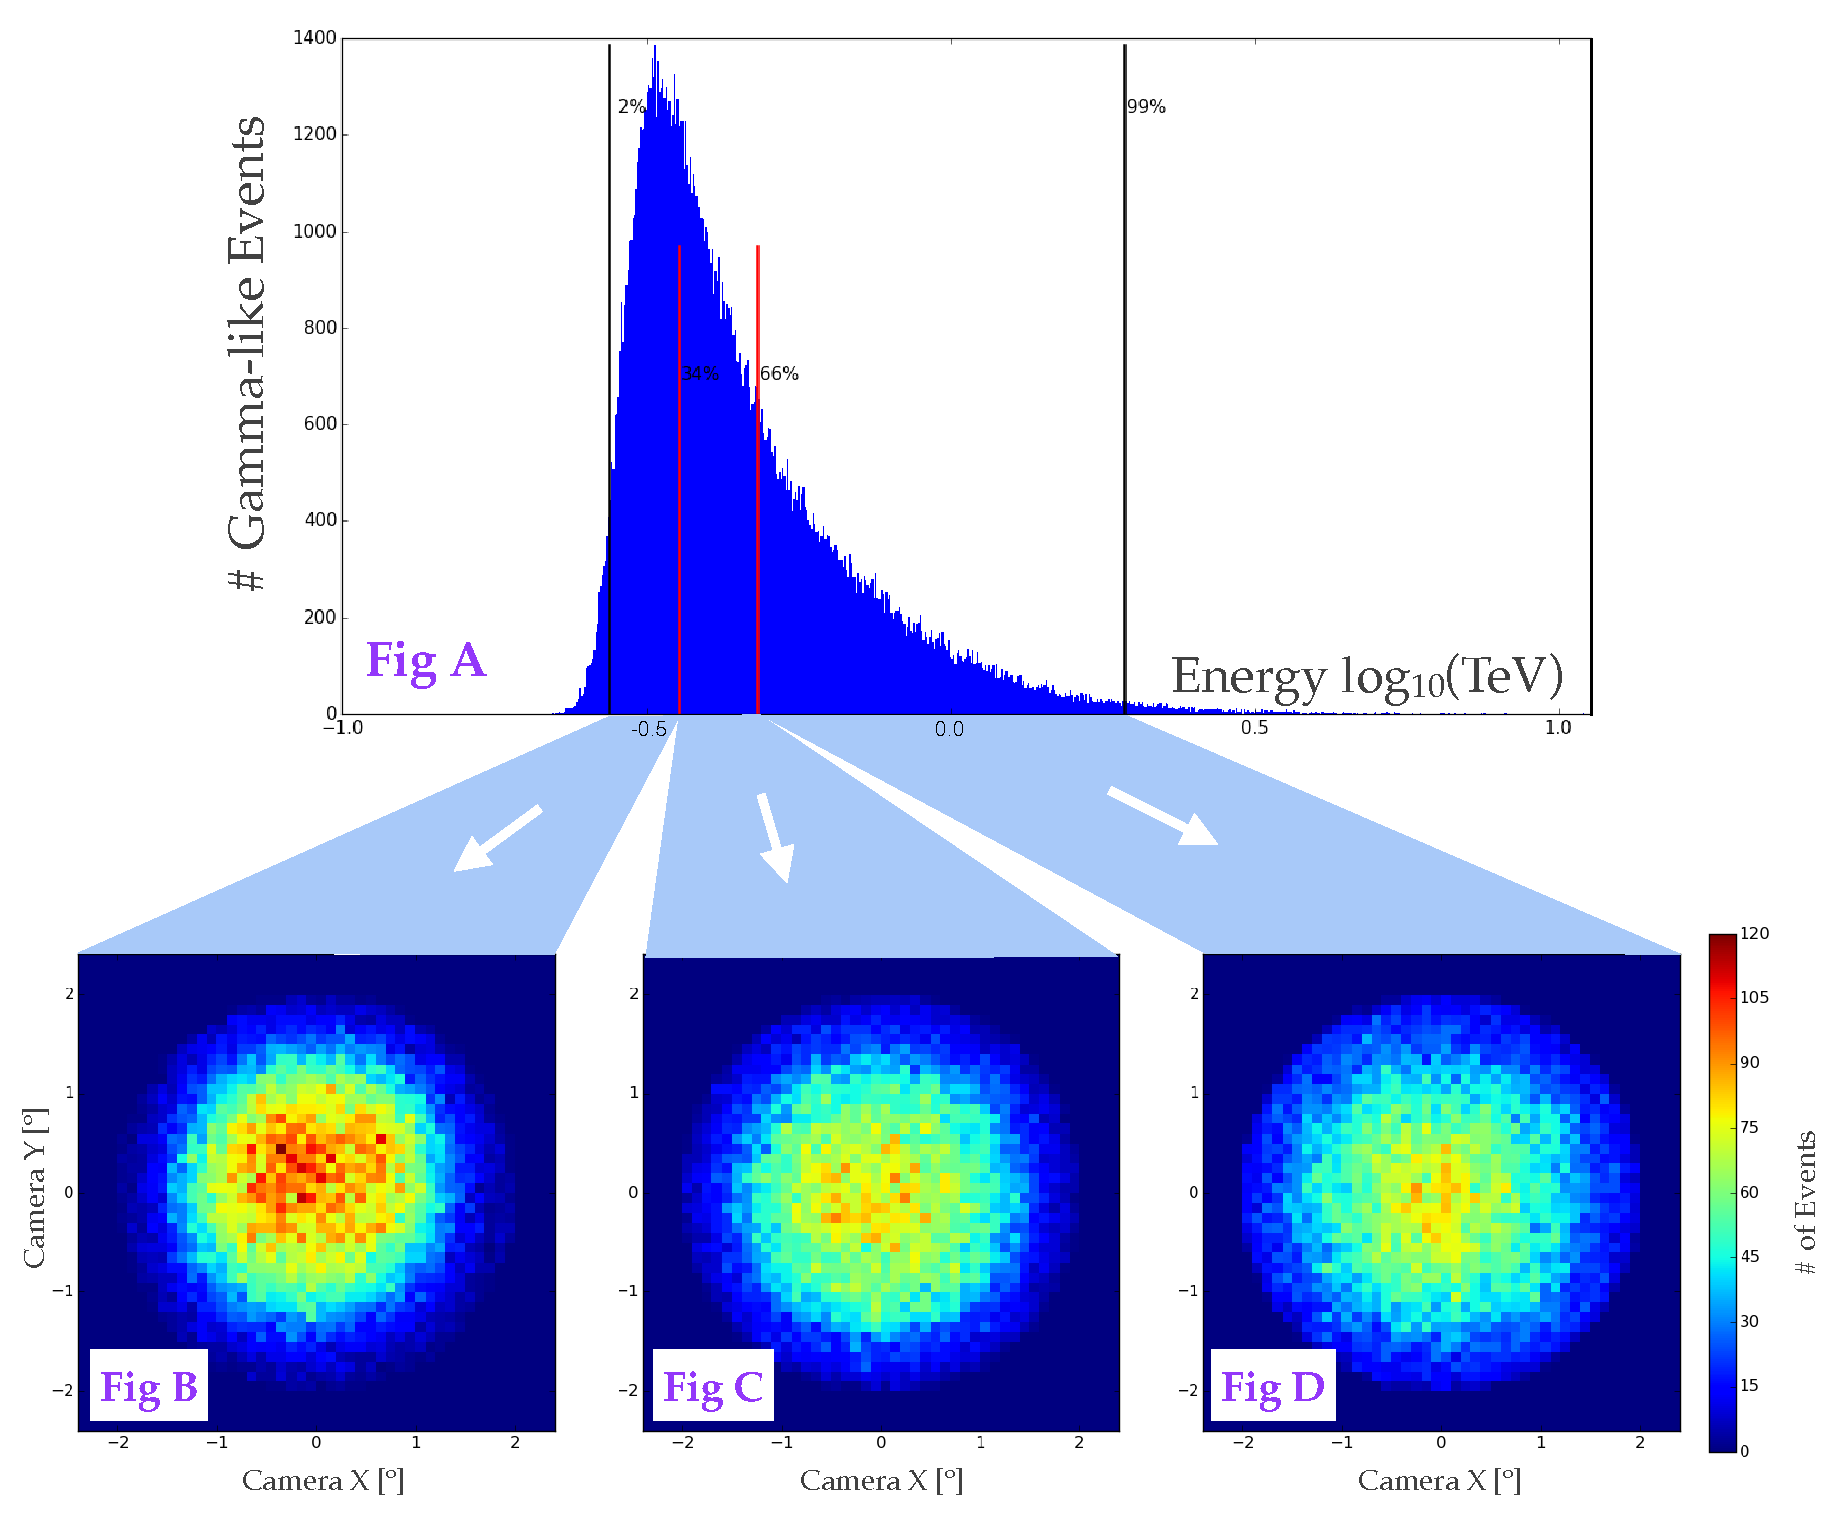
\includegraphics[width=\textwidth]{images/ctools/backgrounds_highelev.eps}
    \caption[FITS Background at 50\degree Elevation]{Gamma-like Events from 52 observations (approximately \nicetilde20 hours) of M82, between 50\degree  and 52\degree  elevations.  Events in Figure A are divided into 3 equal-statistics energy bins, and binned in Camera Coordinates in Figures B, C, and D.}\label{fig:back_highelev}
  \end{center}
\end{figure}

In figure \ref{fig:back_lowelev29} and figure \ref{fig:back_lowelev26}, the same plots are constructed for a set of low-elevation ($ \nicetilde \ang{29} $ and $ \nicetilde \ang{26} $ respectivly)) observations, using Galactic Center Off observations.
These are again divided in to equal-statistic energy bins, and then each energy bin is binned in camera coordinates.
It can be seen that in different energy bins, the background possesses different shapes.

\begin{figure}[ht]
  \begin{center}
    \includegraphics[width=\textwidth]{images/ctools/backgrounds_lowelev29.eps}
    \caption[CTOOLS Background at 29\degree Elevation]{15 Sagittarius A* Off runs (\nicetilde7.5 observation hours), between elevations $ \ang{27.5} $ and $ \ang{30} $.  Events are divided into 6 equal-statistics energy bins, of which four are binned in Camera Coordinates in figures B, C, D, and E.}\label{fig:back_lowelev29}
  \end{center}
\end{figure}

\begin{figure}[ht]
  \begin{center}
    \includegraphics[width=\textwidth]{images/ctools/backgrounds_lowelev26.eps}
    \caption[CTOOLS Background at 26\degree Elevation]{10 Sagittarius A* Off runs (\nicetilde5 observation hours), between elevations $ \ang{24} $ and $ \ang{27.5} $. }\label{fig:back_lowelev26}
  \end{center}
\end{figure}


\subsection{Diffuse Simulations}

To rule out any software causes, diffuse simulations were performed at similar energies and elevations.
These consisted of 50,000 gamma rays at each of 1.4, 1.6, 2, and 5 TeV.
The telescopes were fixed to an azimuth/elevation of (193\degree,28\degree).
The events themselves were distributed in a diffuse disk of radius 2.5\degree.
After having their energy reconstructed, any events falling outside a simple mean-scaled-width cut of -2.0 to 0.5 were removed, which removes many of the proton-induced showers, approximating a gamma-hadron cut.
These are then binned in camera coordinates in figure \ref{fig:back_simdiffuse}.

\begin{figure}[ht]
  \begin{center}
    \includegraphics[width=\textwidth]{images/backgrounds_diffuse_vs_data/diffuse_sims.eps}
    \caption[Diffuse Simulated Backgrounds]{Diffuse simulated gamma-like events in the camera coordinate system at a 28\degree elevation, at 4 different energies.}\label{fig:back_simdiffuse}
  \end{center}
\end{figure}

One can see that the ring and crescent structures persist in these diffuse simulations, implying these are physical effects of the atmosphere and camera, rather than a reconstruction problem.

This striking effect can be seen in Galactic Center data between certain energy ranges.
As the plots are in galactic (l,b) coordinates, and there is a time rotation due to the Earth spinning on its axis, the crescent shapes are still present, albiet smeared around the 4 wobble targets.

plot of galactic center (all energies, ~2TeV energies) !??




